\documentclass[conference]{IEEEtran}

\usepackage[T1]{fontenc}
\usepackage{cite}
\usepackage{amsmath,amssymb}
\usepackage{graphicx}
\usepackage{booktabs}
\usepackage{multirow}
\usepackage[caption=false,font=footnotesize]{subfig}
\usepackage{xcolor}
\usepackage{url}
\usepackage[hidelinks]{hyperref}

\title{ClosRCA-Bench: An Open Topology-Grounded Benchmark and Counterfactual Recovery Framework for Self-Healing Datacenter Networks}

\author{
\IEEEauthorblockN{Dheeraj Ramasahayam}
\IEEEauthorblockA{
\textit{Independent Researcher} \\
United States
}
}

\begin{document}

\maketitle

\begin{abstract}
Open research on datacenter-network root cause analysis (RCA) is limited by two recurring problems: many studies rely on private production traces, and public studies often omit the topology and remediation context needed for self-healing systems. This paper introduces \textit{ClosRCA-Bench}, a reproducible topology-grounded benchmark constructed from Cisco's public Clos-topology telemetry repository by combining event files, CDP maps, and per-device YANG telemetry into fixed graph windows. The resulting benchmark contains 311 windows over 11 topology nodes with 30 features per node and four cause families: BFD outage, blackhole, ECMP change, and interface shutdown. Two fault classes localize to hidden target devices that are not directly monitored, making topology-aware localization a first-class task. The paper evaluates Random Forest, MLP, and a spatio-temporal graph neural network (STGNN) with topology and temporal ablations, and then measures remediation with a safety gate and a counterfactual topology digital twin. On the held-out split, Random Forest achieves the strongest anomaly F1 at 0.9688 and weighted RCA cause F1 at 0.9707. The full STGNN reaches 0.8380 weighted F1 for target-device localization and 1.0000 hidden-target accuracy, while the no-topology ablation collapses to 0.0000 hidden-target accuracy. In the counterfactual recovery twin, gated actions improve mean reachability from 0.9740 under fault to 1.0000 after recovery and achieve 0.8182 recovery-success rate while blocking 100\% of mismatched unsafe actions. The main contribution is therefore an open benchmark and evaluation protocol that makes topology-aware and recovery-aware RCA measurable.
\end{abstract}

\begin{IEEEkeywords}
datacenter networks, root cause analysis, anomaly detection, graph neural networks, network telemetry, self-healing systems, benchmark datasets
\end{IEEEkeywords}

\section{Introduction}
Datacenter networks underpin cloud computing, artificial intelligence training, digital public services, and financial infrastructure. When failures occur, operators need more than alarms; they need fast attribution and a response path that is both effective and safe. This is difficult in practice because symptoms propagate across the topology, measurements are often incomplete, and many remediation actions can make the incident worse if applied to the wrong device.

Recent work has shown that large-scale cloud and datacenter fault localization can be automated to a meaningful degree \cite{roy2017fault,li2021mining}. Graph-based RCA methods have also become more effective at reasoning over dependencies and alert propagation \cite{alertRCA2024,kipf2017semi}. The remaining open problem is not merely model design. It is how to study topology-aware RCA and self-healing behavior on public, reproducible data rather than only on synthetic traces or private incident corpora.

This paper should also be read as deliberately distinct from earlier predictive-maintenance work, including the author's prior attention-guided failure forecasting study \cite{ramasahayam2026prediction}. That earlier work asked whether telemetry can predict failure within a forward warning horizon. The present work addresses a different operational question: once abnormal behavior is present, can a topology-grounded system localize the likely target and recommend an action that survives safety and counterfactual recovery checks?

The paper makes three concrete contributions:
\begin{itemize}
\item \textit{ClosRCA-Bench}, a topology-grounded public benchmark constructed from Cisco Clos-topology telemetry scenarios, event files, and CDP maps \cite{putina2018telemetry,ciscoTelemetryRepo},
\item a spatio-temporal graph RCA model with explicit topology and temporal ablations for hidden-target localization,
\item a safety-gated and counterfactual remediation protocol that measures action correctness, service recovery, and unsafe-action blocking on held-out anomalous windows.
\end{itemize}

\section{Related Work}
Production-oriented datacenter fault detection and localization have been studied in both academic and industrial settings. Roy \textit{et al.} presented passive real-time fault localization for datacenters \cite{roy2017fault}, while Li \textit{et al.} described automated incident detection for cloud services \cite{li2021mining}. These efforts established the operational importance of fast localization, but the underlying data is difficult to reproduce publicly.

Graph-based RCA has become a natural direction because infrastructure failures propagate over dependencies rather than isolated time series. AlertRCA showed that causality-enhanced graph learning improves alert-based RCA \cite{alertRCA2024}, and graph convolutional networks provide an effective message-passing foundation for this class of problems \cite{kipf2017semi}. At the same time, public network telemetry repositories from Cisco have enabled anomaly-detection studies on event-linked network data \cite{putina2018telemetry,ciscoTelemetryRepo}.

The present work is positioned as a benchmark-and-systems paper rather than a claim of a wholly new backbone architecture. Its novelty lies in combining public topology metadata, hidden-target RCA, and counterfactual remediation validation into one reproducible workflow.

\section{Benchmark Construction}
\textit{ClosRCA-Bench} is built from eight public scenarios in Cisco's Clos-topology telemetry collection \cite{ciscoTelemetryRepo}. Each selected scenario includes an event file, a CDP map, and per-device YANG telemetry archives for the monitored subset of devices. We retain four fault families:
\texttt{bfd\_outage}, \texttt{blackhole}, \texttt{ecmp\_change}, and \texttt{interface\_shutdown}.

The construction pipeline performs four steps. First, it parses per-device telemetry archives and extracts compact device-level features from data-rate, generic-counter, BFD, BGP, FIB-drop, interface-state, and CPU collections. Second, it aligns samples into 10-second bins and builds a fixed graph whose nodes are routers in the Clos fabric. Third, it labels anomaly intervals directly from the event files. Fourth, it converts each scenario into 60-second graph windows with a 30-second step.

Two target devices, \texttt{leaf3} and \texttt{spine4-3464}, are not directly present in the monitored telemetry subset. They are nevertheless retained as localization labels because the topology exposes their adjacency to the observed nodes. This makes hidden-target localization measurable rather than implicit.

\begin{figure}[t]
\centering
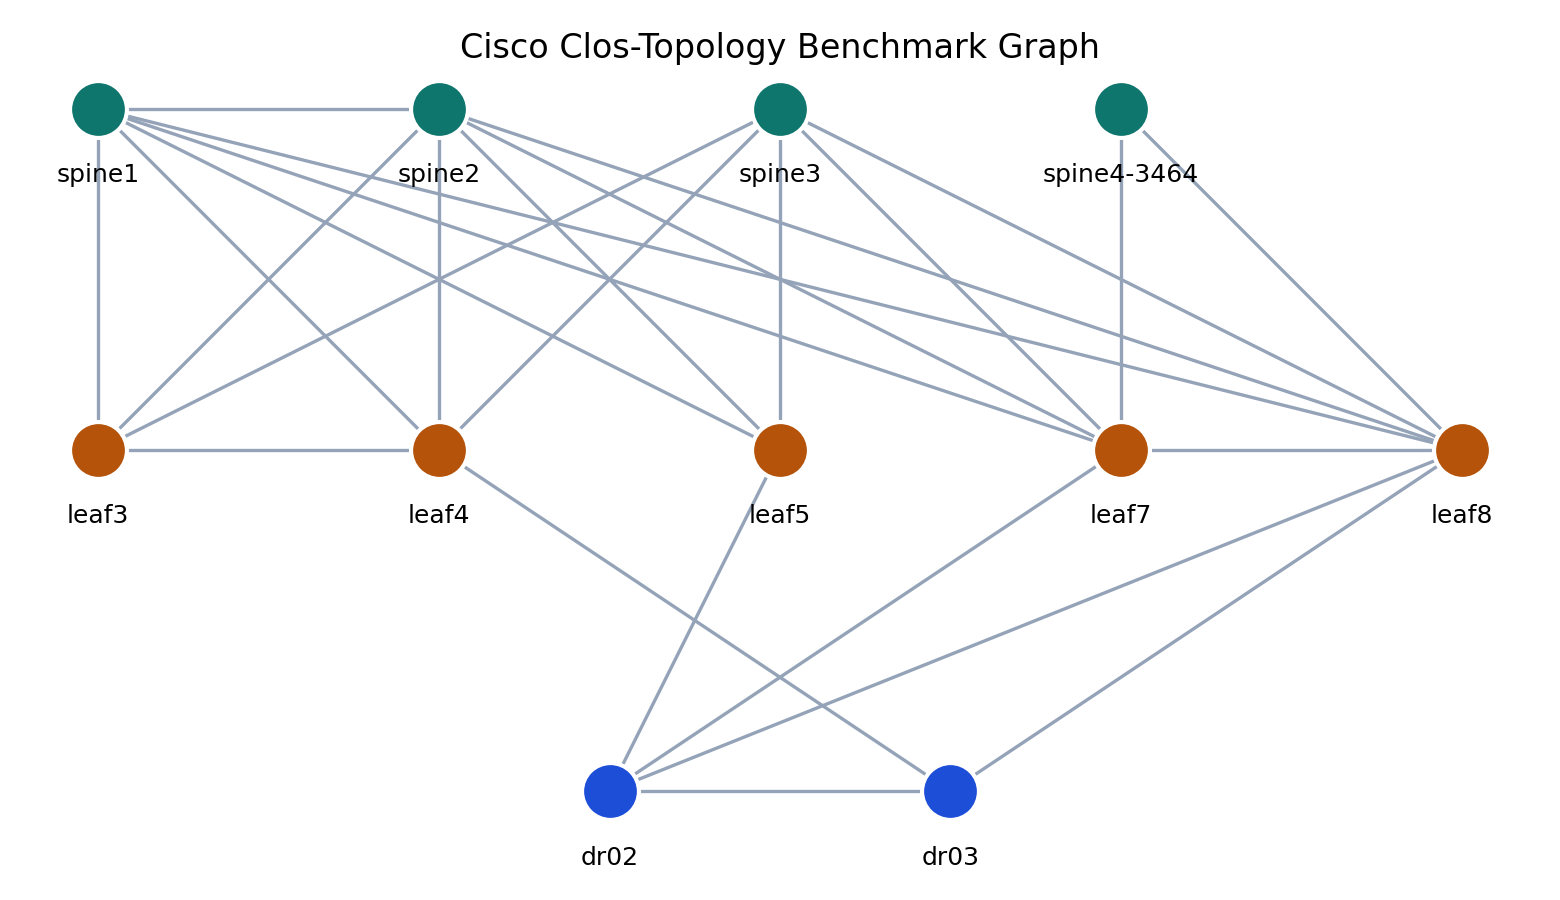
\includegraphics[width=\columnwidth]{graphs/cisco_clos_topology.png}
\caption{Topology graph used by the public Cisco Clos-topology benchmark. Hidden-target labels include \texttt{leaf3} and \texttt{spine4-3464}.}
\label{fig:topology}
\end{figure}

\begin{table}[t]
\caption{Benchmark Summary}
\label{tab:dataset}
\centering
\begin{tabular}{lc}
\toprule
Property & Value \\
\midrule
Scenarios & 8 \\
Cause families & 4 \\
Graph nodes & 11 \\
Features per node & 30 \\
Window size & 6 bins (60 s) \\
Window step & 3 bins (30 s) \\
Total windows & 311 \\
Normal windows & 147 \\
Anomalous windows & 164 \\
Hidden target devices & 2 \\
\bottomrule
\end{tabular}
\end{table}

The benchmark supports three tasks:
\begin{itemize}
\item binary anomaly detection over graph windows,
\item multiclass cause classification over anomalous windows,
\item target-device localization over anomalous windows.
\end{itemize}

\section{Model and Recovery Twin}
The proposed RCA model is a spatio-temporal graph neural network (STGNN). Each graph window is a tensor of shape \((T, N, F)\), where \(T\) is time, \(N\) is the number of topology nodes, and \(F\) is the per-node feature count. A GRU encodes each node's temporal behavior, graph convolution propagates state across the topology, and three heads predict anomaly, cause class, and target device.

The target-localization head is intentionally topology-aware. Instead of predicting only from a pooled graph embedding, it scores the candidate target nodes directly after message passing. This is important for hidden-target scenarios because the candidate device may have no direct telemetry but can still be inferred from neighboring symptoms.

Two ablations are evaluated:
\begin{itemize}
\item \textbf{No topology}: replace the graph adjacency with the identity matrix,
\item \textbf{No temporal}: replace temporal encoding with a mean-pooled projection.
\end{itemize}

The paper also evaluates two strong graph-free baselines, Random Forest and MLP, on flattened graph windows.

Remediation is evaluated in two stages. First, a safety gate validates whether an action is allowed on the predicted target and whether it respects simple topology constraints such as alternate-path availability for interface reroutes. Second, a lightweight topology digital twin scores the counterfactual effect of the action on service reachability, path diversity, overload, and blast radius. Each predicted cause-target pair maps to an action template such as \texttt{restore\_bfd\_session}, \texttt{rollback\_blackhole\_route}, or \texttt{reroute\_and\_restore\_interface}. This converts remediation from advisory text into a measurable recovery stage.

\section{Results}
Table~\ref{tab:results} reports the held-out benchmark metrics. Random Forest is strongest overall on anomaly detection, cause classification, and aggregate target-device localization. This is an important benchmark result in its own right: the public benchmark is not a guaranteed deep-learning win. The STGNN nevertheless shows a clear topology-specific advantage on the hidden-target slice, which is the benchmark setting where topology should matter most.

\begin{table*}[t]
\caption{Held-Out Benchmark Performance}
\label{tab:results}
\centering
\begin{tabular}{lccccc}
\toprule
Model & Anomaly F1 & Cause F1$_w$ & Target F1$_w$ & Hidden-Target Accuracy & Unsafe Blocked \\
\midrule
Random Forest & 0.9688 & 0.9707 & 1.0000 & 1.0000 & -- \\
MLP & 0.8438 & 0.9707 & 0.9702 & 1.0000 & -- \\
STGNN Full & 0.8182 & 0.9532 & 0.8380 & 1.0000 & 1.0000 \\
STGNN No Topology & 0.7931 & 0.9524 & 0.6566 & 0.0000 & -- \\
STGNN No Temporal & 0.7931 & 0.9532 & 0.6646 & 0.9000 & -- \\
\bottomrule
\end{tabular}
\end{table*}

The topology effect is clearest in target localization. On the full anomalous test slice, the STGNN improves target-device weighted F1 from 0.6566 in the no-topology ablation to 0.8380. On the hidden-target subset, the full model reaches 1.0000 accuracy while the no-topology ablation falls to 0.0000. This indicates that message passing is doing useful work specifically where direct telemetry is unavailable.

The remediation layer reaches 0.8485 action-match rate, 0.8485 safety-pass rate, and blocks 100\% of mismatched unsafe actions on held-out anomalous windows. In the counterfactual recovery twin, the same gated actions improve mean service reachability from 0.9740 in the injected-fault state to 1.0000 after recovery, reduce mean blast radius by 0.0260, and achieve 0.8182 recovery-success rate. In other words, the gate does not merely mirror the classifier. It suppresses bad actions, and the digital twin translates that suppression into measurable recovery outcomes.

\begin{figure}[t]
\centering
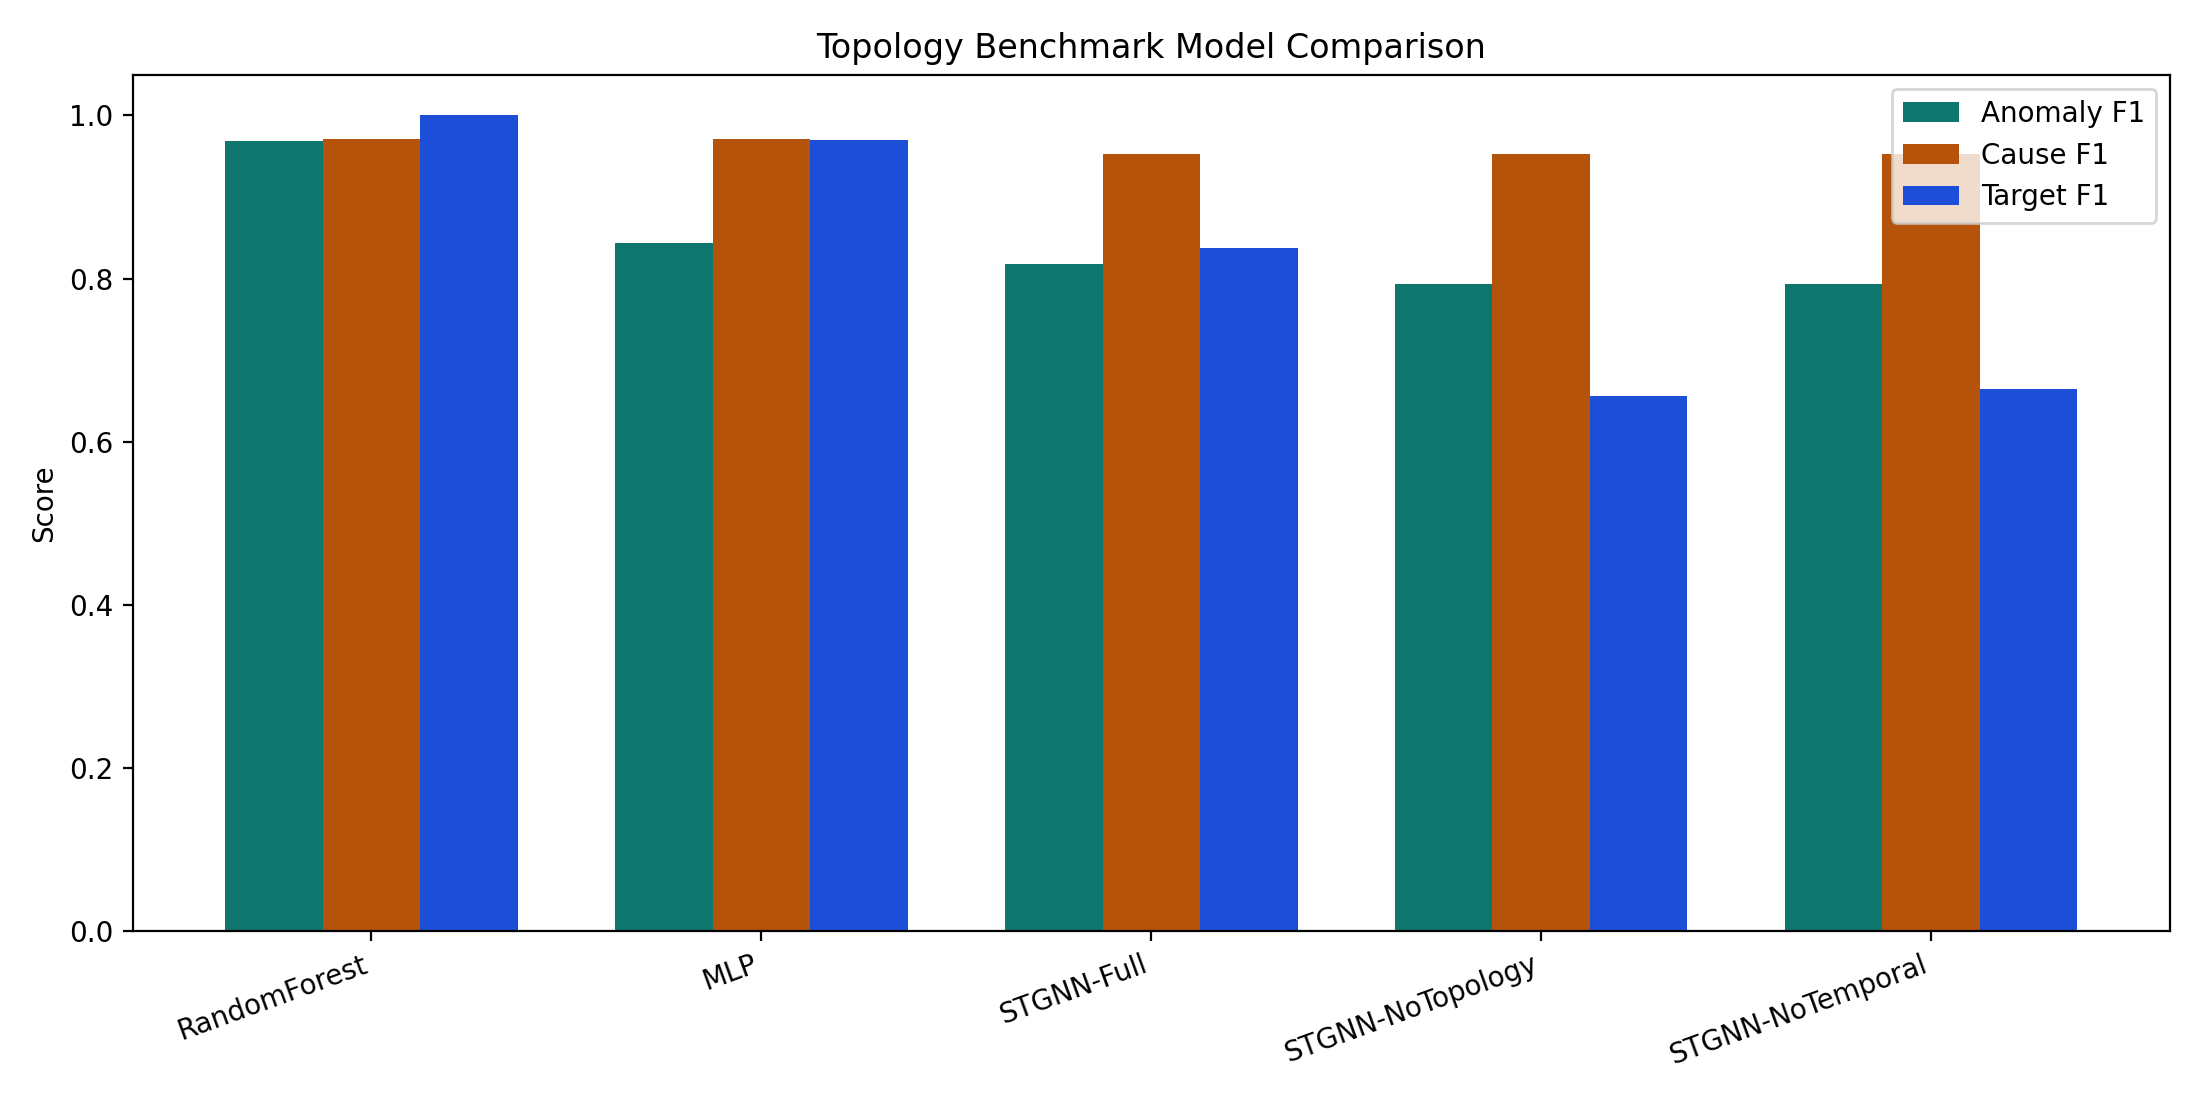
\includegraphics[width=\columnwidth]{graphs/topology_model_comparison.png}
\caption{Held-out comparison of anomaly, cause, and target metrics on the topology-grounded benchmark.}
\label{fig:modelcompare}
\end{figure}

\begin{figure}[t]
\centering
\subfloat[STGNN ROC]{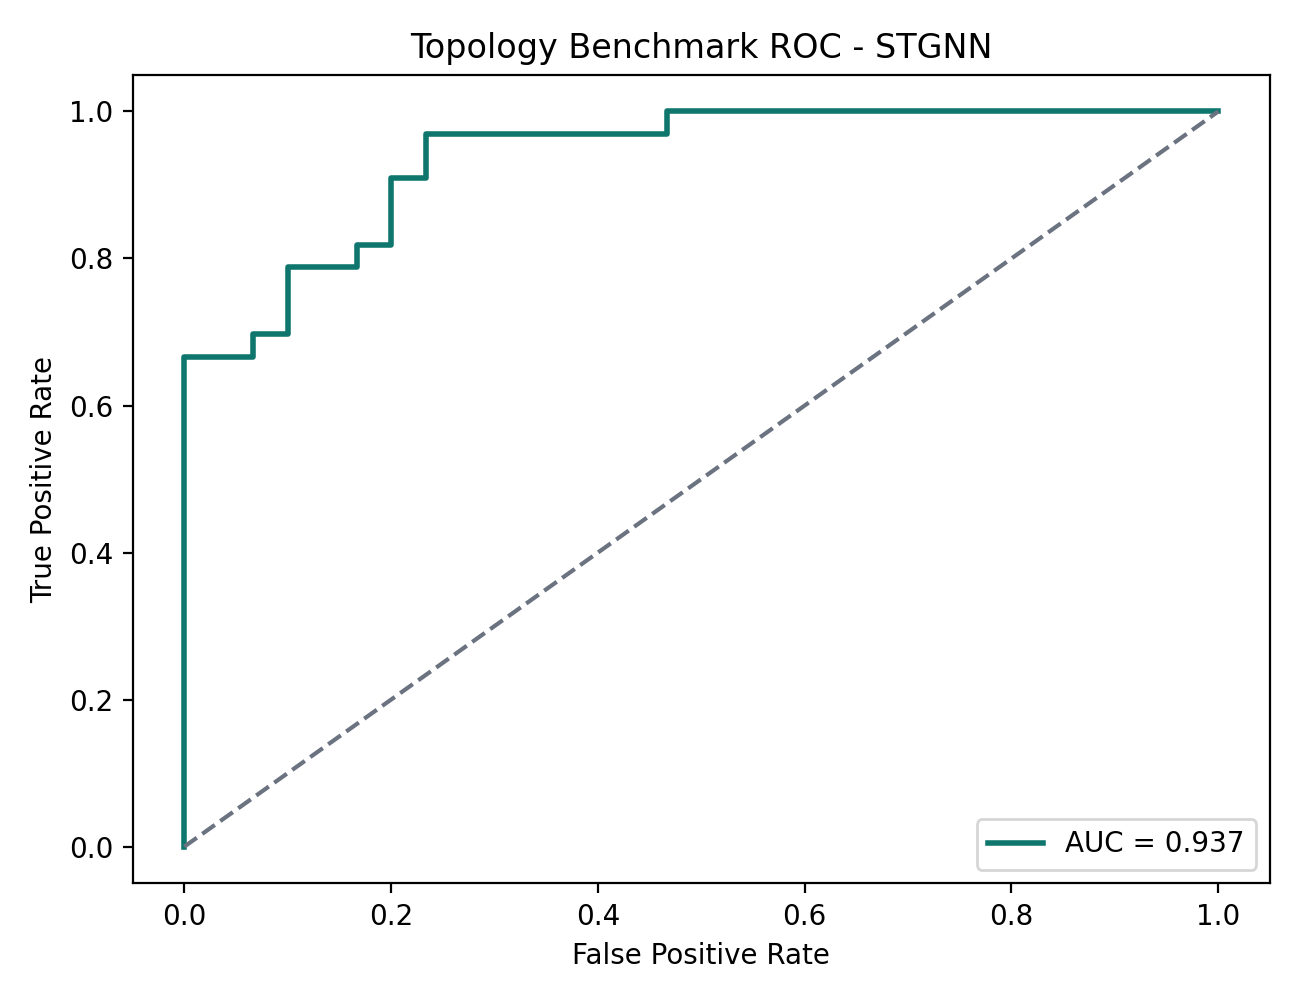
\includegraphics[width=0.48\columnwidth]{graphs/topology_stgnn_roc.png}\label{fig:rocstgnn}}
\hfill
\subfloat[Target confusion matrix]{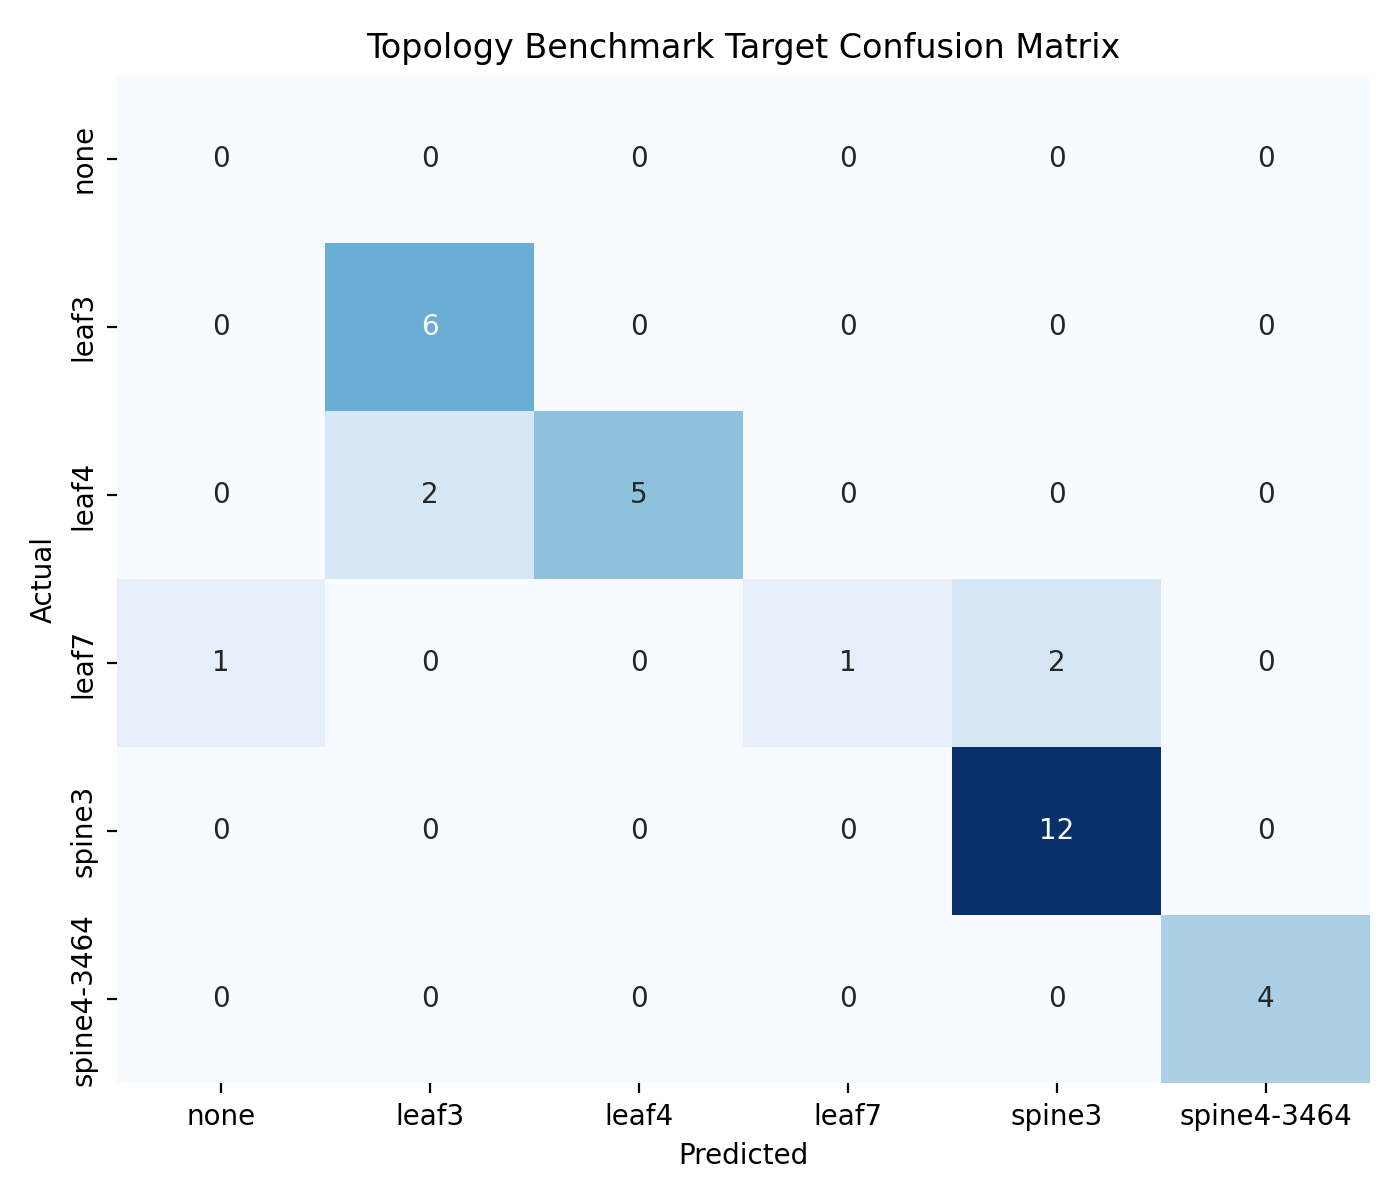
\includegraphics[width=0.48\columnwidth]{graphs/topology_target_cm.png}\label{fig:cmtarget}}
\caption{Held-out anomaly and target-localization diagnostics for the full topology model.}
\label{fig:diagnostics}
\end{figure}

\begin{figure}[t]
\centering
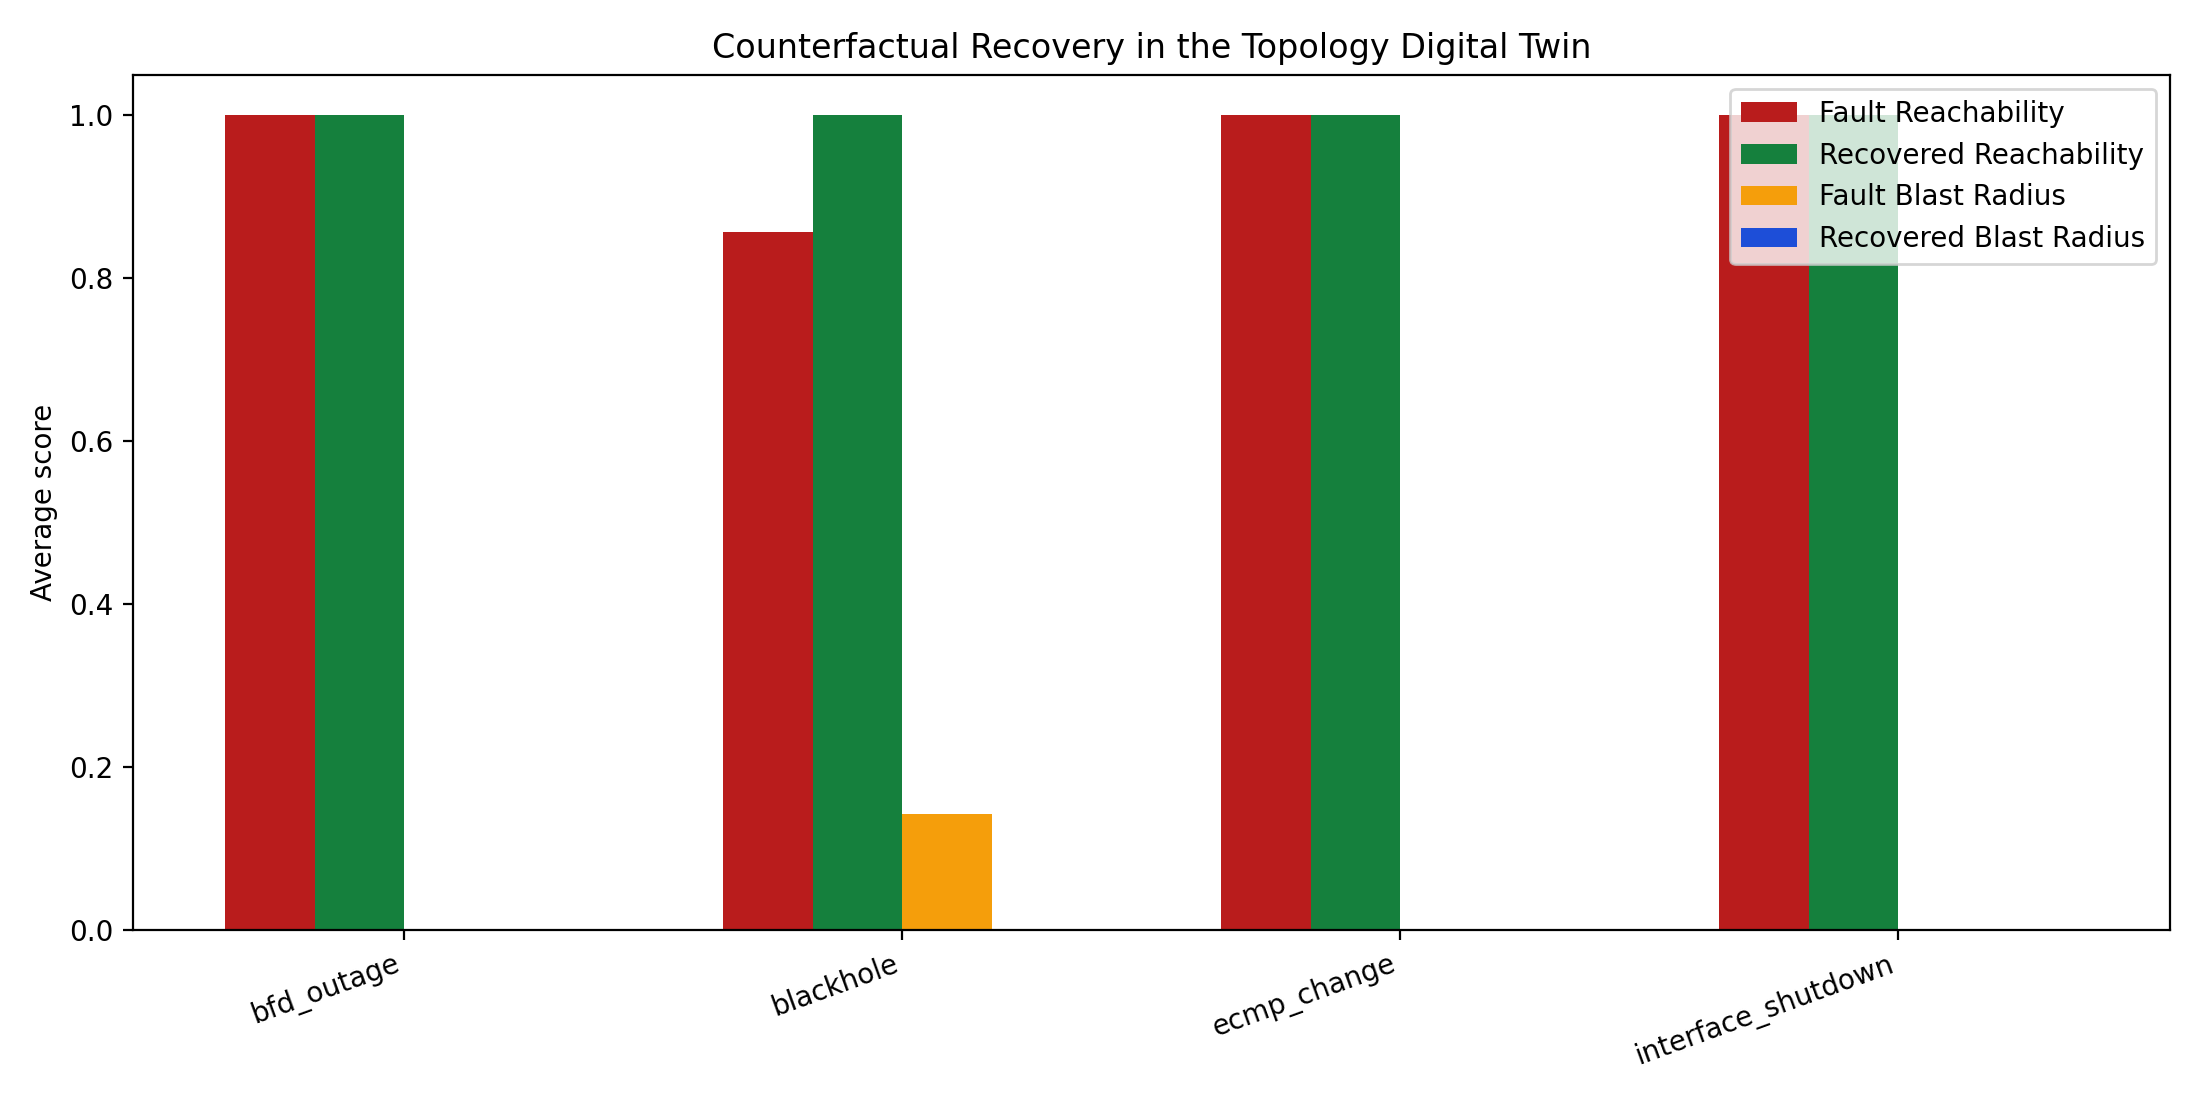
\includegraphics[width=\columnwidth]{graphs/topology_digital_twin_recovery.png}
\caption{Counterfactual recovery results in the topology digital twin, grouped by fault family.}
\label{fig:digitaltwin}
\end{figure}

\section{Discussion and Limitations}
Three observations matter most. First, benchmark construction is the primary scientific contribution here. The value is not that the STGNN beats every baseline; it is that topology-aware and recovery-aware RCA can now be studied on public data with fixed artifacts and hidden-target labels. Second, the topology signal appears where it should: not in easy aggregate classification, but in localizing devices without direct telemetry. Third, the recovery twin makes remediation measurable. A paper about self-healing should report not only whether a classifier is correct, but whether the proposed action improves network state under a counterfactual replay.

The current benchmark still has clear limits. It covers only eight scenarios from one lab topology. The network-loop scenario in the public repository was not included because the unpacked directory does not expose the per-device telemetry archives needed by the current parser. The recovery twin is a lightweight topology simulator rather than a controller-in-the-loop emulator such as containerlab or Batfish. Finally, strong classical baselines remain difficult to beat on the aggregate metrics, so future work should focus on harder scenarios, richer labels, and live-control validation.

\section{Conclusion}
This paper reframes the project around a stronger and more defensible thesis: public topology-grounded benchmarking plus counterfactual recovery validation for self-healing datacenter networks. \textit{ClosRCA-Bench} exposes hidden-target localization, supports reproducible anomaly and RCA evaluation, and measures remediation quality explicitly through both safety gating and a topology digital twin. The topology-aware STGNN is most useful where topology should matter most, namely hidden-target localization, while the recovery layer blocks unsafe actions and quantifies service restoration. The next step is to expand the benchmark with additional public scenarios and validate the action layer against a live network emulator.

\bibliographystyle{IEEEtran}
\bibliography{references}

\end{document}
